\documentclass[10pt,conference,compsocconf]{IEEEtran}
\usepackage{hyperref}
\usepackage{graphicx}   % For figure environment
\usepackage{subfigure}
\usepackage{titling} % Customizing the title section
\usepackage{dblfloatfix}    % To enable figures at the bottom of page
\usepackage{kantlipsum}     % for random text
\usepackage{todonotes}
\usepackage{multirow}
\usepackage[margin=0.9in]{geometry}
\usepackage[english]{babel}
\usepackage{caption,setspace}

\usepackage{dsfont}

\usepackage{array}
\newcolumntype{P}[1]{>{\centering\arraybackslash}p{#1}}
\newcolumntype{M}[1]{>{\centering\arraybackslash}m{#1}}
\begin{document}
        
\pretitle{\begin{center}\Huge\bfseries} % Article title formatting
\posttitle{\end{center}} % Article title closing formatting
\title{Hotgrad: a deep learning framework}
\author{
        % Your name
        \textsc{Niccol\`{o} Sacchi, Succa Riccardo \& Marco Zoveralli}
        \normalsize{} \\
        % Your institution
        \normalsize \'{E}cole polytechnique f\'{e}d\'{e}rale de Lausanne
}
\maketitle
\begin{abstract}
This project aims to design and implement a simple deep learning framework based only on pytorch Tensors and standard math libraries. Such a framework consists in implementing backward compliant operations so that, by applying the chain rule, we can compute all the needed gradients. We achieved this goal by implementing forward and backward functions for the basic operations, i.e. (1) operations between two tensors (e.g. matrix multiplication) and (2) operations on a single tensor input (e.g. ReLU). This approach lead to a straightforward implementation of all the needed operations while keeping the framework versatile and easy to understand.
This framework had been tested by implementing a simple neural network trained on a two dimensional dataset and comparing the performace with some baselines.
\end{abstract}
\section{Introduction}
A neural network consists in a series of layers, which compute a linear mapping of their input. In order to improve the capacity of the model, non-linear functions are usually introduced after each linear layer. These non-linear functions avoid that the output of the network can be reproduced from a linear combination of the input, which leads to poor accuracy when the input dataset is not linearly separable (classification) or the target is not linearly dependent on the input (regression).
When a neural network is created, its parameters are randomly initialized; therefore, in a 2-class cassification problem, the accurancy of the network is initially around 50\%. The latter is improved during the learning phase which is based on three main steps repeated for a certain number of iterations: (1) the \textit{forward pass}, (2) the \textit{backward pass} and (3) \textit{parameters update}. 
\begin{enumerate}
    \item The forward pass can just be seen as a series of function applied in sequence to the input in order to compute the output of the network $y$: \[y = f(g(h(...(x)))\]
    \item Then a loss function is used to measure how much the output of the network differs from the expected output. The backward pass computes the gradients of the loss with respect to the network parameters by applying the chain rule.
    \item Finally, all the computed gradients are used to update the respective network parameters with the final goal of minimizing the train loss. For example, the stochastic gradient descent uses the following formula to update a parameter: \[parameter = parameter + \eta\nabla L(parameter)\]
\end{enumerate}
In a fully connected layer the trainable parameters consist in the weights and the biases and it is implemented with the following formula (X represents a single input sample):
\[y = X*W + b\]
 $ \mbox{where } X \in \mathbb{R}^{1*M} 
 \mbox{, } W \in \mathbb{R}^{M*D} 
 \mbox{, } b \in \mathbb{R}^{1*D}
 \mbox{ and } y \in \mathbb{R}^{1*D} $ 

These general steps can be applied to any differentiable structure. It is therefore important for a deep learning framework to be easy to use and highly versatile so that various operations can be freely combined in order to construct both simple and more complex neural networks. Our approach focused on these features and aimed to implement the more complex operations (e.g. linear layer, MSE loss) by breaking them into basic operations between tensors and making them backward compliant by simply implementing their gradient.

Section \ref{sec:Implementation} introduces the main ideas behind the design of the frameworks. Section \ref{sec:CodeStructure} shows in details the code implementation and the module's structure. Section \ref{sec:Test} compares our solution with some baselines and with a similar network built with the pytorch library. Section \ref{sec:Future} summerizes our achievements and focus in some possible future developments.
        
% All the weights and biases of the network are initially set to a uniform value from the interval $(-1/\sqrt{d}, 1/\sqrt{d}) $ (where d is the layer's input dimension),
\section{Implementation}
\label{sec:Implementation}
Since this project provided the structure of the final neural network, a simple approach to the problem would have been to directly implement the forward and the backward for the whole network. This would lead to a simple but difficult-to-read implemetation, without any possibility to expand or modify the network. We immediately discarded this option and we instead focused on a modular approach.
The backward propagation can be easily computed by iteratively applying the chain rule and propagating the computed gradients starting from the very last operation, i.e. the loss. The following (simplified) formula shows how the chain rule is applied to compute the gradient of a composite function:
\[\delta_w(f(g(w))) = \delta_{g(w)}(f(g(w)))*\nabla_w(g(w))\]
$\mbox{where } g: \mathbb{R}^{M*N} \rightarrow \mathbb{R} \mbox{ and } f: \mathbb{R} \rightarrow \mathbb{R}. $ \\
Particular attention has to be payd to the shapes of the tensors when applying this formula. With this in mind, we understand that to be able to propagate the gradients all the way back to the parameters we need to store all the acyclic graph of operations that lead from the input to the computation of the loss. We achieve this goal with two simple ideas:
\begin{itemize}
    \item Each operations should keep track of its inputs other than computing the result of the operation. In this way each operation can compute the derivative of its output with respect to its input, multiply it with the current gradient and pass it to it(s) input(s).
    \item In turn, each operand should (1) be able to propagate the gradient to the operation that computed the operand itself and (2) store the received gradient (which represents the gradient of the loss with respect to the operand) which will be possibly used to update this parameter during the parameter update phase. We achieved this by implementing a class called \textit{Variable} to wrap all the necessary information: the operand itself (which consists in a torch FloatTensor), its gradient and the link to the operation that generated it.
\end{itemize}
This structure allows to perform both the forward and backward passes. In the \textbf{forward pass}, each operation takes its inputs Variables and produces a new output Variable which contains the resulting tensor, a gradient tensor initialized to zeros and the link to the operation itself. Then, this new Variable can be used as input for any subsequent operation, and the process is repeated. Starting from the input, this chain of operations continues until the computation of the loss. In the \textbf{backward pass}, each operation receives the gradient from its output Variable, i.e. the gradient of the loss with respect to it, and multiply it with the gradient of the output Variable with respect to each input Variable. The obtained gradients are finally passed to the relative input Variables. Whenever a Variable receives a gradient, it is accumulated in its \textit{gradient} field and then passes it to the previous operation if any.
With this structure in mind, we implemented the base operations, i.e. the activation functions ReLU and Tanh, and addition, subtraction, element-wise multiplication, matrix multiplication, pow and mean. This can be seen as a bottom up approach, where we break the problem into very basic operations, and then use them to construct more complex modules. The graph shown in figure \ref{fig:ForwardBackward} displays how this modules and variables are used to compute the forward and backward pass.

\begin{center}
	\label{fig:ForwardBackward}
	\captionsetup{type=figure}
	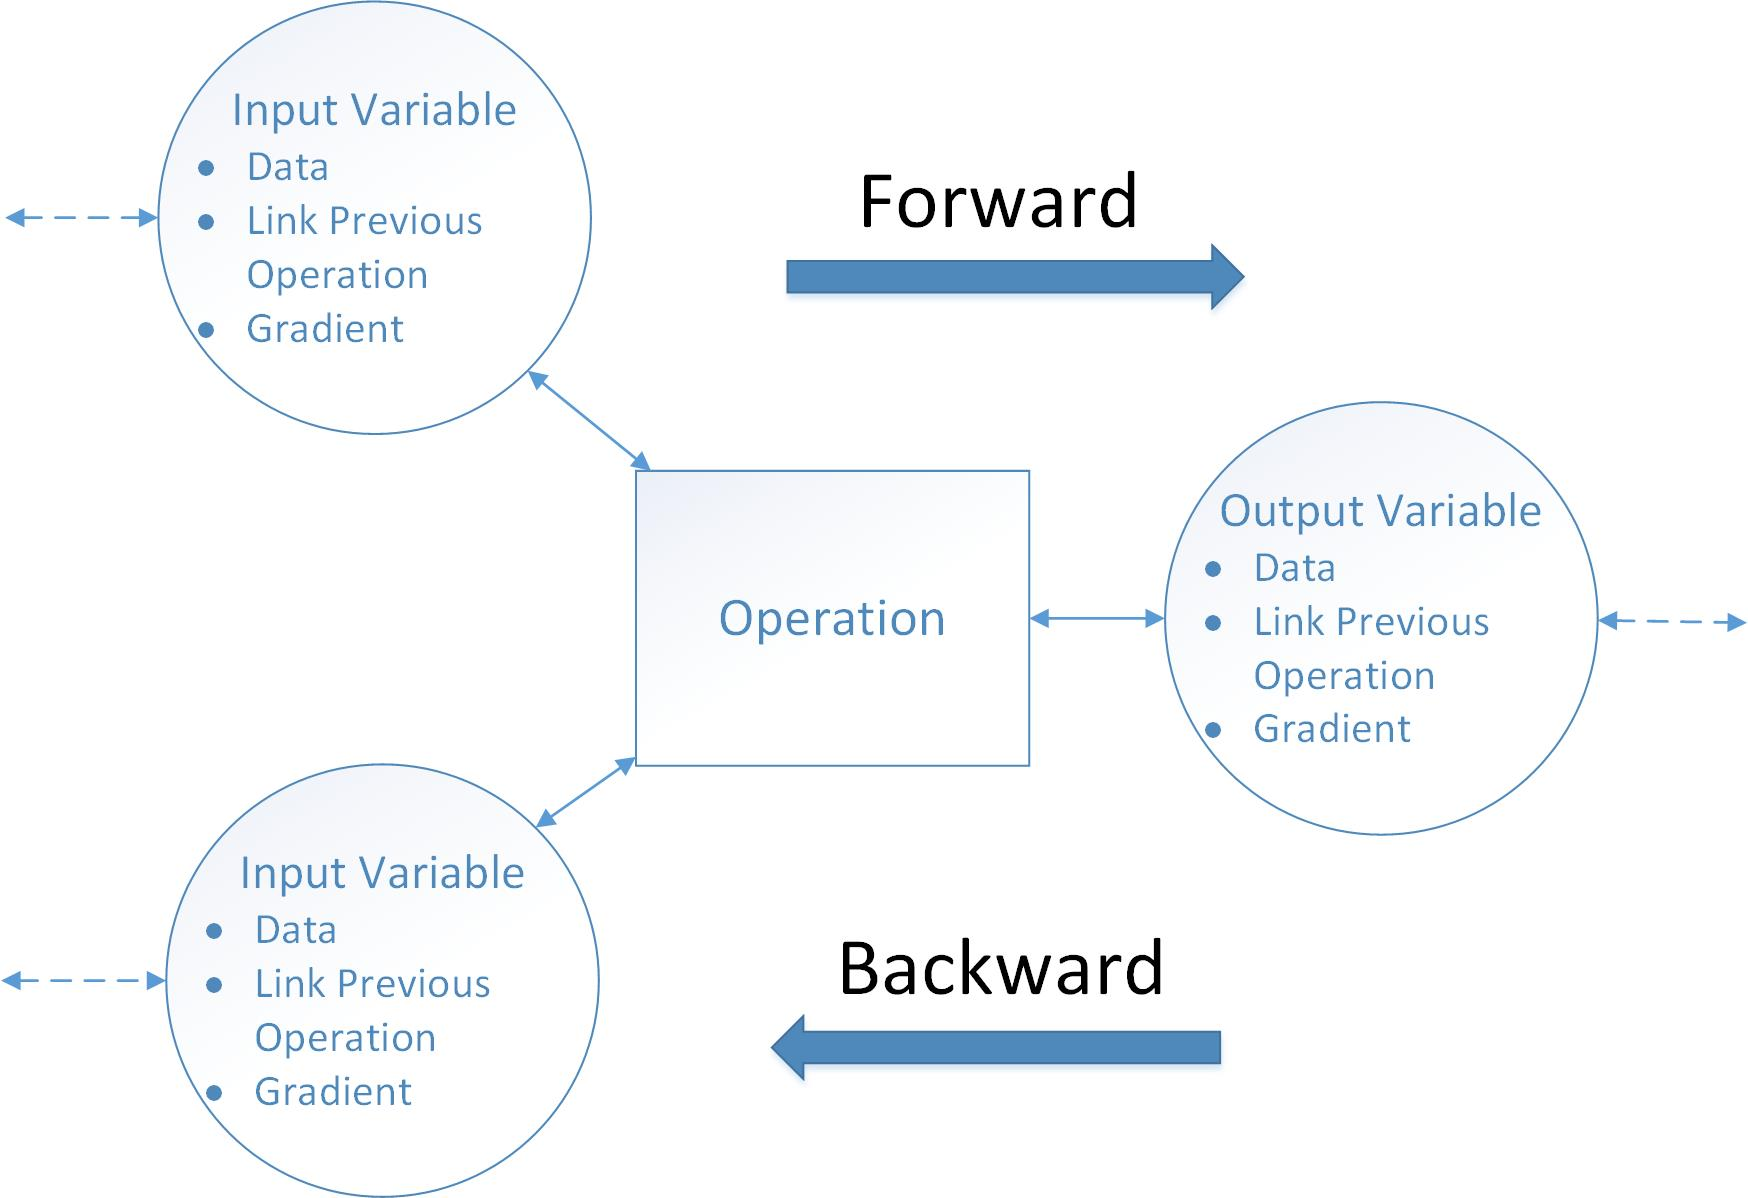
\includegraphics[width=0.5\textwidth]{img/ForwardBackward.jpg}
	\caption {Forward: The Operation Module generates a new Variable, containing the result and the link to the opration itself. Backward: The Operation Module computes the new gradients and sends them to the respective Input Variables.}
\end{center}        
        
\section{Code Structure}
\label{sec:CodeStructure}
We now describe in details the structure of the code and the classes you can find in our library folder \textit{hotgrad}:

\begin{table*}
	\caption{Modules}
	\label{tab:modules}
	\begin{tabular}{ | c | c | p{10cm} | c | } 
		\hline
		Module & Classes & Description & Forward  \\
		\hline
		\multirow{2}{4em}{Activations} 
		& ReLU & Implements the rectified linear unit, extending the Module1Operands & $f(x) = max(0, x)$  \\
		& Tanh & Hyperbolic tangent function that extend the Module1Operands & $f(x) = tanh(x)$ \\
		\hline
		\multirow{6}{4em}{Operands}
		& Add & \multirow{6}{30em}{All these classes extend Module2Operands or Module1Operands depending on the number of inputs. They implement the forward and backward pass. } & $f(x, y) = x + y$ \\
		& Sub & & $f(x, y) = x - y$ \\ 
		& Mul & & $f(x, y) = x \odot y$ \\ 
		& MatMul & & $f(x, y) = x * y$ \\ 
		& Pow & & $f(x, exp) = x^{exp}$ \\ 
		& Mean & & $\frac{1}{N} \sum_{i=1}^N x_i$ \\
		\hline
		Layers & Linear & The Linear module is a wrapper of two operation: multiplication of the weights and sum of the biases. & $f(x) = w*x + b$ \\ 
		\hline
		Losses & MSE & The mean square error extend the Module2Operands & $\frac{1}{N} \sum_{i=1}^N (x_i - \overline{x})^2$  \\ 
		\hline
	\end{tabular}
\end{table*}

\begin{itemize}
	\item \textit{module.py}: this file contains the abstract class Module, with the basic funcions that each module will implement, in particular the forward and backward pass. This Module class is extended by two other classes, Module2Operands and Module1Operand, that distinguish between operations that respectively require one or two inputs. 
	
	\item \textit{exception.py}: contains the exceptions needed to handle the errors.
	
	\item \textit{optimizers.py}: as optimizer, we implemented the Stocastic Gradient Descend (SDG), initialized with a learning rate parameter. The method \textit{set\_params} allows to register the list of all the trainable network parameters, whose update is performed by the \textit{step} function.
	
	\item \textit{sequential.py}: this module is used as a container of other modules. It receives as input the list of modules that compose the network, the loss criterion and the optimizer. Unlike the other modules, Sequential does not implement the backward pass. It has a \textit{fit} method that is used to train the network on a given train data and for a specified number of epochs. Each epoch correspond on a pass on the whole training data. In order to speed up the performance by updating more often the parameters, the \textit{batch\_size} specifies on how many samples we estimate the gradient before the parameters update step. In this way, the parameters are optimized every batch size and not with the entire train set.
	
	\item \textit{variable.py}: this class is the wrapper class for the torch FloatTensor. It stores:
	\begin{itemize}
        \item \textit{data}: a FloatTensor representing the value of the variable.
		\item \textit{grad}: a FloatTensor representing the accumulated gradient of the loss with respect to this variable.
		\item \textit{requires\_grad}: boolean used to indicate whether we have to use the \textit{grad} to update the \textit{data} during the parameter update step.
		\item \textit{previous\_op}: is the link to the operation which generated this Variable.
	\end{itemize}
	
	\item \textit{functions.py}: this folders contain different modules that implements the basic functions. Table \ref{tab:modules} describes its content in details.
\end{itemize}

We also added support for the broadcasting functionality, which is the possibility of repeating a FloatTensor on one dimension in order to allow certain matrix operations. This functionality is for example used in the Linear module, when the bias is added to the result obtained from the multiplication between the input and the weight matrix. In the forward pass, this operation is trivially handled by the broadcast property of pytorch Tensors. However, in the backward pass, the gradient received by the broadcasted Variable has not the same size of its data field. We have to simply sum the gradient tensor on the replicated dimension before adding in with the Variable's grad. This operation derives from the mathematical property:
\[\frac{d}{dx}f(x,y)|_{x=y} = \frac{d}{dx}f(x,y) + \frac{d}{dy}f(x,y)\]
When a variable is broadcasted, the dimensions that are expanded contains replicated values, which refers to the constraint $x=y$ of the above formula. Consequently, the derivative of the gradient can be seen as the sum of the derivatives along the axes that were replicated.

Table \ref{tab:modules} summarizes the modules that are implemented in our framework, along with a short description and a specification of the forward pass:


\section{Tests and Results}
\label{sec:Test}
%next steps and conclusions 
% indexing, convolutional
In this section we provide the description of the dataset and the network built with our framework. Then, the validity of the built model is shown by comparing it with well-known baselines.

\subsection{Dataset}
The dataset consists of a training set and a test set of 1000 points each. These points are sampled uniformly in [0, 1], and they are labeled with -1 if they end up out of the disk of radius \( \frac{1}{\sqrt{2\pi}} \) and center (0.5, 0.5), with label 1 otherwise. The following exhibit - which represents the train set used during the testing phase - contains a set of points that satisfy these properties:

\begin{center}
	\captionsetup{type=figure}
	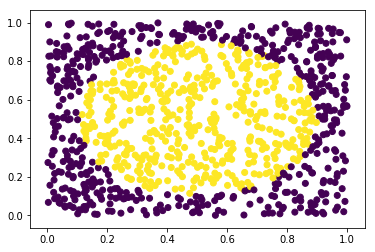
\includegraphics[width=0.5\textwidth]{img/dataset.png}
	\label{fig:dataset}
\end{center} 

For the sake of reproducibility, we used a manual seed to ensure that all the runs of the test would be the same.

\subsection{Network}
The network consists of two input units, two output units and three hidden layers of 25 units.

\begin{center}
	\captionsetup{type=figure}
	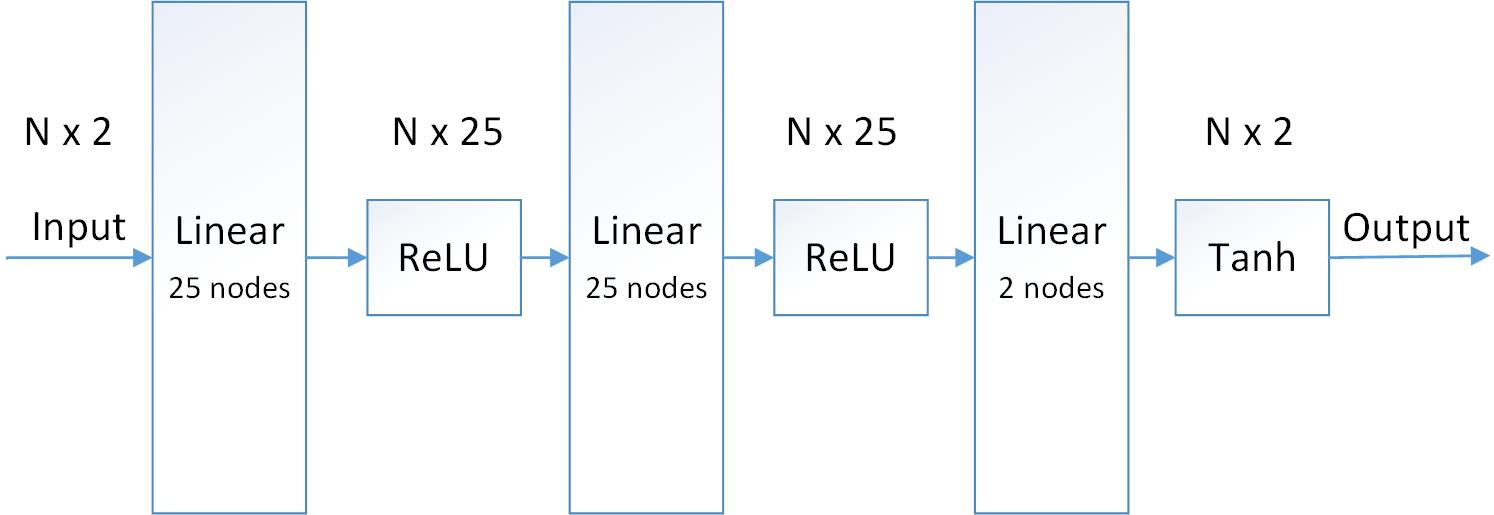
\includegraphics[width=0.5\textwidth]{img/Network.jpg}
	\label{fig:network}
\end{center} 

A Tanh activation function is used as the last component of our network. The reason behind this choice is that having an unbounded output in a classification problem where MSE is used, would highly penalize both very positives and very negatives outcomes. In fact, the true labels can only have two values and if the network output is unbounded any value that is either too high or too small is interpreted, by the MSE function, as something very different from the labels. By using the Tanh this problem is mitigated as the output of the network is bounded to [-1, 1]. The predicted target values are obtained by is approximating the output to the closest label.

\subsection{Model Comparison}
Our model had been tested on the aforementioned dataset. The results are quite satisfying, since the test accuracy is around 98\%.
%The following image compares our model with common baselines.
A comparison of our model with some common baselines and the same model built by using the pytorch library is shown below:
\begin{center}
	\captionsetup{type=figure}
	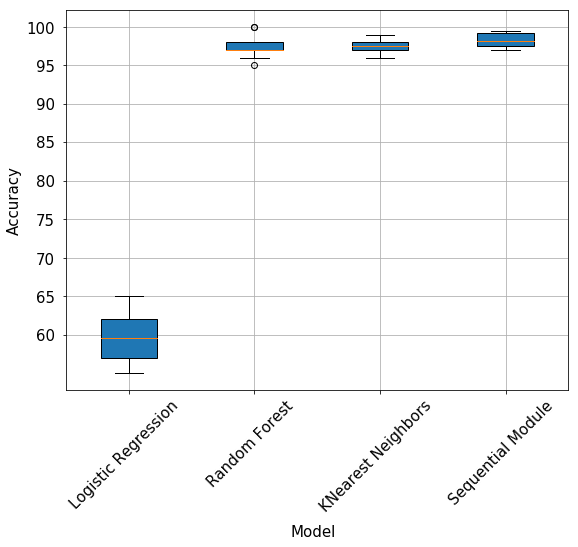
\includegraphics[width=0.5\textwidth]{img/boxplots_final.png}
	\label{fig:boxplot}
\end{center} 
Intuitively, as expected, non-linear classifers, e.g. K-NN, random forest, perform reasonably well, while linear ones, e.g. logistic regression, give the worst result because the points in the dataset are not linearly separable. With the latter models, higher performance can be achieved only through feature extraction. It can also be seen that our model performs slightly better than any of the tested baselines.

Finally, it is we can notice that the the sequential module built by using our framework gives very similar accuracies as the one built by using the pytorch primitives.

\section{Future developments and Conclusions}
\label{sec:Future}
We designed and implemented a functioning deep learning framework which allows to easily develop additional features such as loss functions, optimizers, layers by provinding their respective backward pass. Some improvements could be brought, e.g. the backward propagation stops only when a Variable with no previous operation receives the gradient and stops propagating it, this could potentially correspond to a waste of computation as these Variables usually do not require any gradients.
%The goal of this project was to design a fully connected neural network, but the framework can be easily expanded to support convolutional layers. The latters are beyond the complexity of the problem, but they would have been useful if we had to classify images and not simple points.

\end{document}
